\documentclass{article}

\usepackage[top=3cm, bottom=3cm, left=3cm, right=3cm]{geometry}

\usepackage[utf8]{inputenc}
\usepackage[T1]{fontenc}
\usepackage[frenchb]{babel}

\usepackage[a4paper,colorlinks,linkcolor=darkgray,citecolor=red,urlcolor=blue]{hyperref}
\usepackage{graphicx}
\usepackage{caption}
\usepackage{subcaption}
\usepackage{amsthm}
\usepackage{listings}
\usepackage{tikz}
\usepackage{algorithm}
\usepackage{amsmath}
\usepackage[noend]{algpseudocode}
\usepackage{amsfonts}
\usepackage{amssymb}
\usepackage{authblk}

\renewcommand\Affilfont{\small}

\title{Projet Images}

\author[$\dag$]{Laureline Pinault et Raphaël Charrondière}
\affil[$\dag$]{ENS de Lyon, France}

\date{Lundi 4 mai 2015}

\begin{document}

  \maketitle

  \begin{abstract}
   
  \end{abstract}
  
  \newpage

  \tableofcontents

  \newpage
  
  \section{Introduction}
  
    \subsection{Remarques préliminaires}
    
    \subsection{objectifs du projet}
  
    \subsection{Organisation du projet}
  
  \section{Traitement des images}
  
    \subsection{Traitement anti-inversion}
  
    \subsection{Traitement anti-bruit}
    
    \subsection{Remplissage}
    
      \begin{figure}[!h]
	\centering
	\begin{subfigure}{.25\textwidth}
	  \centering
	  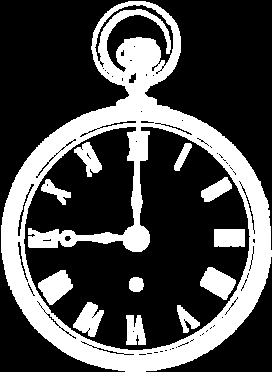
\includegraphics[scale=0.30]{Illustrations/pocket-20.png}
	  \label{pocket-non-rempli}
	\end{subfigure}
	\begin{subfigure}{.25\textwidth}
	  \centering
	  
\includegraphics[scale=0.30]{Illustrations/pocket-20-rempli.png}
	\label{pocket-rempli}
	\end{subfigure}
	\caption{}
	\label{remplissage}
      \end{figure}
      
      \begin{figure}[!h]
	\centering
	\begin{subfigure}{.25\textwidth}
	  \centering
	  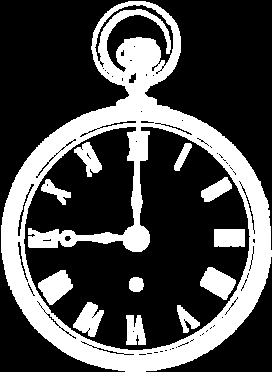
\includegraphics[scale=0.30]{Illustrations/pocket-20.png}
	  \label{pocket-non-rempli}
	\end{subfigure}
	\begin{subfigure}{.25\textwidth}
	  \centering
	  
\includegraphics[scale=0.30]{Illustrations/pocket-20-rempli.png}
	\label{pocket-rempli}
	\end{subfigure}
	\begin{subfigure}{.25\textwidth}
	  \centering
	  
\includegraphics[scale=0.30]{Illustrations/pocket-20-rempli.png}
	\label{pocket-rempli}
	\end{subfigure}	
	\caption{}
	\label{remplissage}
      \end{figure}      
   
  \section{Estimateurs}
  
    \subsection{Quelques estimateurs simple et complémentaires}

      \subsubsection{Solidité}
      
      \subsubsection{Exentricté}
      
      \subsubsection{Energie de flexion moyenne}
    
    \subsection{Transformée de fourrier}
    
    \subsection{}
  
  \section{Résultats}
  
\end{document}

